\documentclass[conference]{IEEEtran}
\IEEEoverridecommandlockouts
\usepackage{amsmath,amssymb,amsfonts}
\usepackage{algorithmic}
\usepackage{graphicx}
\usepackage{textcomp}
\usepackage{xcolor}
\usepackage{pgfplots}
\pgfplotsset{compat=1.18}
\usepackage{pgfplotstable}
\usepackage{caption}
\usepackage{siunitx}
\usepackage{multirow}
\usepackage{booktabs}
\usepackage{tikz}
\usepackage{orcidlink}
\usepackage{flushend}
\hypersetup{pdfborder={0 0 0}}

\usetikzlibrary{positioning, shapes.geometric, arrows.meta, calc}
\def\BibTeX{{\rm B\kern-.05em{\sc i\kern-.025em b}\kern-.08em
    T\kern-.1667em\lower.7ex\hbox{E}\kern-.125emX}}

\begin{document}

\title{Internship Report - Code Generation with Vision Language Models for Robot arms application.}

\author{
\IEEEauthorblockN{
Tran Quang Minh\,\orcidlink{0009-0001-2238-2180},
Luu Trong Hieu\,\orcidlink{0009-0001-3953-3133},
Nguyen Cong Khanh\,\orcidlink{0009-0005-6197-7565},
Nguyen Quang Trung\,\orcidlink{0009-0005-5265-2208}
}
\IEEEauthorblockA{
\textit{Department of Artificial Intelligence} \\
\textit{FPT University | VietDynamic JSC}\\
Ho Chi Minh City, Vietnam\\
Emails: quantran102005@gmail.com, Luutronghieu0709@gmail.com, congkhanhtruongthi@gmail.com, trungnqse183108@fpt.edu.vn
}
}
\maketitle

\begin{abstract}
This report presents the internship experience of our team, who worked on a project titled "Code Generation with Vision Language Models for Robot arms application." The internship took place at VietDynamic JSC from September 2025 to December 2025. The primary objective of the project was to explore the capabilities of vision language models (VLMs) in generating code for robot arm applications. The report details the tasks undertaken, challenges faced, and the skills acquired during the internship. It also highlights the significance of VLMs in automating code generation and their potential impact on the robotics industry. We express our gratitude to VietDynamic JSC for providing this valuable learning opportunity. 
Code is available at: \href{https://github.com/Minhtrna/Code-gen-for-robot-arm-OJT-FALL-2025-FPT}{GitHub/Code-gen-for-robot-arm-OJT-FALL-2025-FPT}
\end{abstract}

\section{Introduction}
The rapid advancement of artificial intelligence (AI) and machine learning has led to the development of vision language models (VLMs) that can understand and generate human-like text. These models have shown remarkable capabilities in various natural language processing tasks, including code generation. The ability to generate code automatically has significant implications for the software development industry, particularly in specialized fields such as robotics.
During our internship at VietDynamic JSC, we had the opportunity to work on a project focused on leveraging VLMs for code generation in robot arm applications. The project aimed to explore how VLMs can assist in automating the coding process, thereby improving efficiency and reducing the time required for software development in robotics.
This report provides a comprehensive overview of our internship experience, including the tasks we undertook, the 
challenges we encountered, and the skills we developed. We also discuss the potential applications of VLMs in the robotics industry and their impact on future developments.

\section{Related Work}
Recent advancements in large language models (LLMs) have demonstrated their potential in various applications, including code generation for robotic systems. Notable works in this domain include Mu et al.'s RoboCodeX\cite{mu2024robocodex}, which explores the use of LLMs to generate code for robotic tasks, showcasing the ability of these models to understand and execute complex instructions. Another significant contribution is the Robotic Programmer by Xie et al.\cite{xie2025robotic}, which focuses on video-instructed policy code generation for robotic manipulation, highlighting the integration of visual inputs with LLMs to enhance robotic capabilities. These studies underscore the transformative potential of LLMs in automating and optimizing code generation for robotics, paving the way for more efficient and intelligent robotic systems.
Other relevant works include the development of vision-language models (VLMs) like MobileVLM\cite{chu2023mobilevlm}, which are designed to handle multimodal inputs, making them suitable for applications that require both visual and textual understanding. The integration of VLMs in robotics can significantly enhance the interaction between robots and their environments, enabling more sophisticated and context-aware behaviors.

\section{Methodology}
\subsection{Overview}
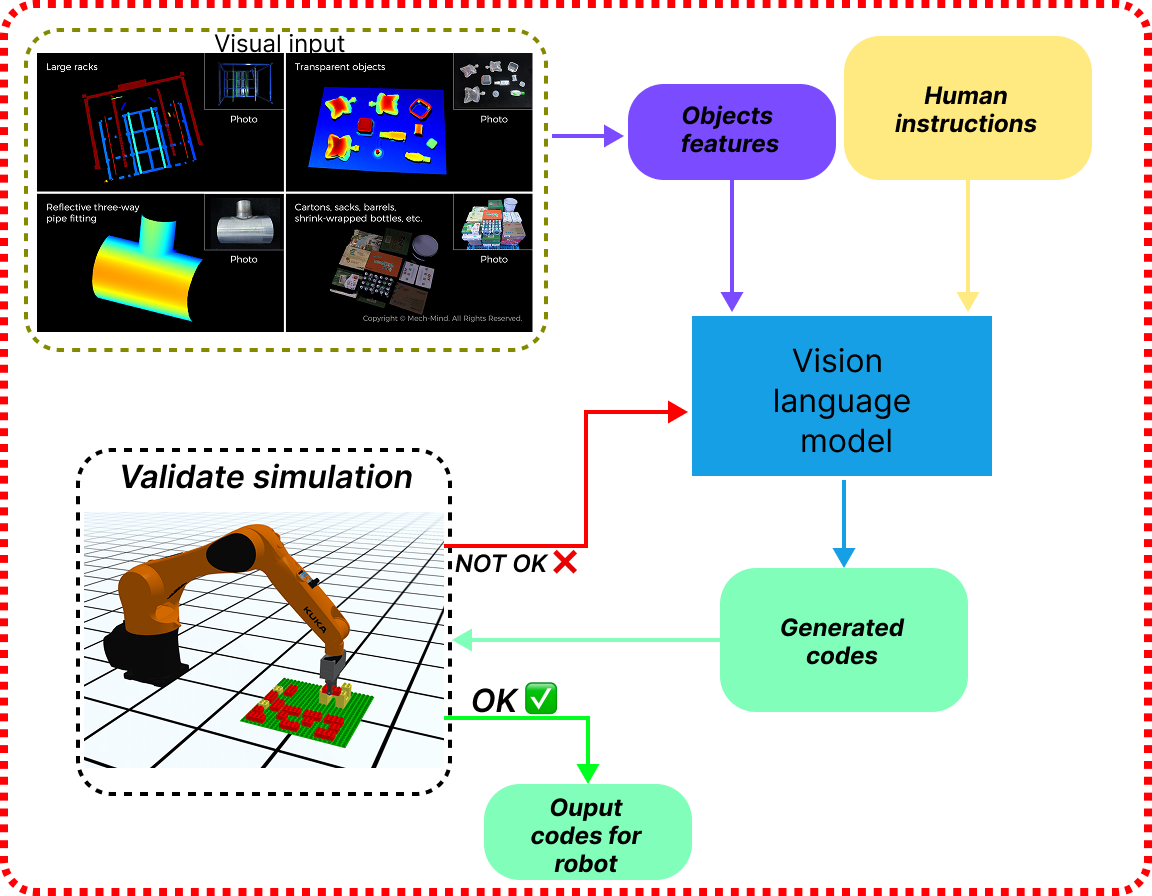
\includegraphics[width=7cm]{OJT_fig_1.png}

We leverage the capabilities of vision language models (VLMs) to generate code for robot arm applications. Combined with visual information from dedicated sensors like Mech-EYE we could enhance the understanding of the environment and improve the accuracy of the generated code. 
The overall pipeline consists of several key components: Mech-EYE 3D industrial camera, VLMs, and a simulator for validating the generated code without the need of physical hardware. The Mech-EYE camera captures high-resolution images and 3D point clouds of the robot's surroundings, providing essential visual context for the VLMs. The VLMs, such as MobileVLM or specialized models like RoboCodeX\cite{mu2024robocodex}, are then employed to generate code based on the visual data and specific task requirements. More comprehensive tasks such as video instructions for robotic manipulation are also considered \cite{xie2025robotic}.
Finally, the generated code is executed in a controlled environment built with \href{https://docs.ros.org/}{ROS2} and \href{http://gazebosim.org/}{GAZEBO} to validate its functionality and performance.
\subsection{Systems Design}
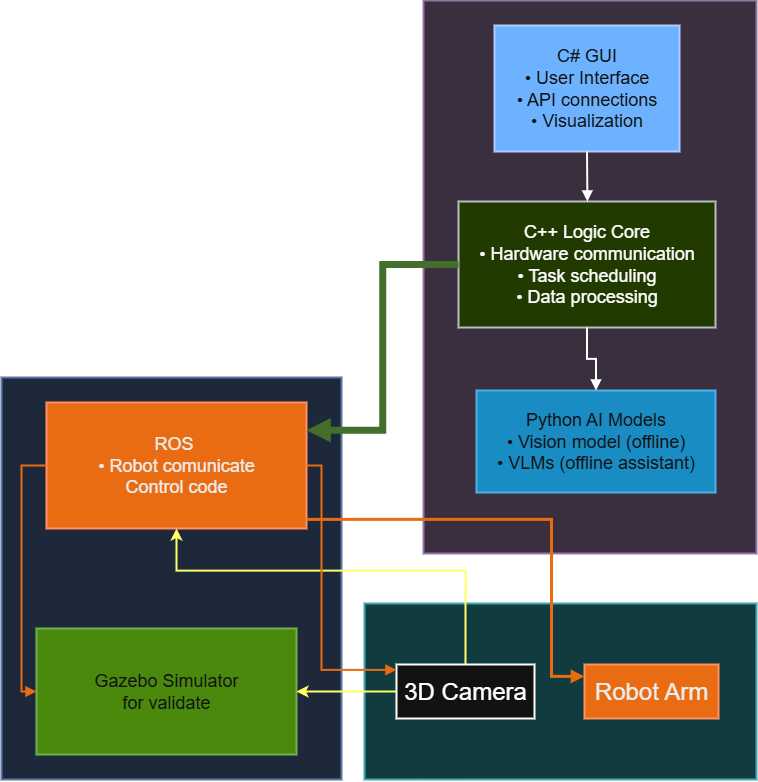
\includegraphics[width=8cm]{Design.png}

We designed a modular system architecture to facilitate the integration of various components involved in the code generation process.
The architecture consists of the following modules:
\begin{itemize}
    \item \textbf{GUI Module:} This module is responsible for user interaction. It allows users to input task specifications, view visual data from the Mech-EYE or Intel Realsense cameras, and monitor the code generation process.
    user can also select the VLM they want to use for code generation, do work with camera like calibration, capturing image, point cloud, etc.
    \item \textbf{Logic Core Module:} This module manages the communication with the various system components, ensuring smooth data flow and coordination between modules. It also handles all Logic task like communication with hardwares, processing user inputs, data, etc.
    \item \textbf{VLM and Vision Integration Module:} This module interfaces with the selected vision language models and vision models. It handles the input of visual data and task specifications, and it retrieves the generated code from the models. 
    \item \textbf{Simulate and Validate Module:} This module let user simulate and assess the performance of the generated code based on predefined metrics such as accuracy, efficiency, and robustness. It provides feedback for further refinement of the VLMs generated code and the overall system.
\end{itemize}   

\subsection{Vision Language Models}

Robotic team is responsible for the integration and fine-tuning of the vision language models (VLMs) used for code generation. They ensure that the selected VLMs are properly configured to handle the specific requirements of robot arm applications.
The team also works on optimizing the performance of the VLMs by fine-tuning them on relevant datasets and adjusting hyperparameters to improve code generation accuracy.
We plan to use MobileVLMV2\cite{chu2024mobilevlm} as the base model for our code generation tasks due to its efficiency and effectiveness in handling multimodal inputs. The model will be fine-tuned on a custom dataset of robotic tasks to enhance its performance in generating context-aware code.
The VLM will be integrated into the system to provide real-time code generation capabilities, allowing for
dynamic adaptation to changing task requirements and environmental conditions.

MobileVLMV2\cite{chu2024mobilevlm} is a vision-language model that combines the strengths of both visual and textual data to perform various tasks, including image captioning, visual question answering, and code generation. The model is designed to be lightweight and efficient, making it suitable for deployment on devices with limited computational resources.
Compared to the older version MobileVLM\cite{chu2023mobilevlm}, MobileVLMV2\cite{chu2024mobilevlm} introduces several improvements, including enhanced model architecture, better training techniques, and increased robustness to various input types. These enhancements lead to improved performance across a range of tasks while maintaining the model's efficiency.
Figure \ref{fig:latency-comparison-mobile} shows the comparison of SOTA VLMs in terms of average performance across several standard benchmarks and speed (tested on an NVIDIA Jeston Orin with lamma.cpp). MobileVLMV2 achieves new state-of-the-art results with much faster inference speed. Figure \ref{fig:model-scaling} shows the scaling of MobileVLMV2 model, which demonstrates that as the model size increases, the performance on various benchmarks also improves, indicating the effectiveness of the model architecture and training approach, compared to its predecessor.
\begin{figure}[t]
  \centering
   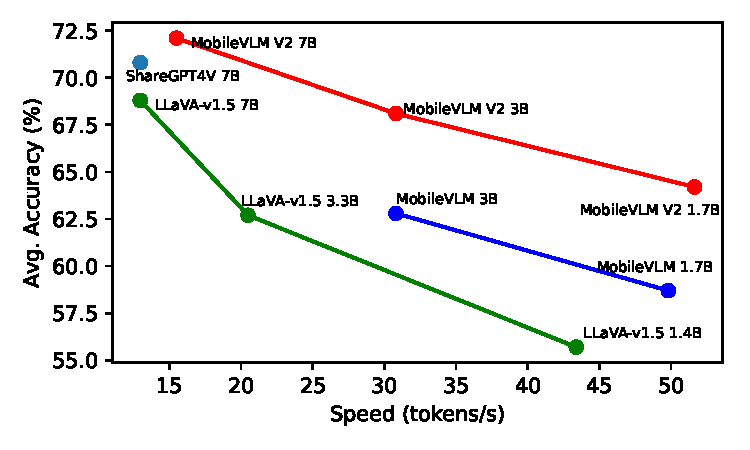
\includegraphics[width=.87\columnwidth]{figures/mobilevlm_latency_mobile.pdf}
   \caption{Comparison of SOTA VLMs in terms of average performance across several standard benchmarks and speed (tested on an NVIDIA Jeston Orin with lamma.cpp). MobileVLMV2 achieves new state-of-the-art results with much faster inference speed.}
   \label{fig:latency-comparison-mobile}
\end{figure}

\begin{figure}[ht]
  \centering
   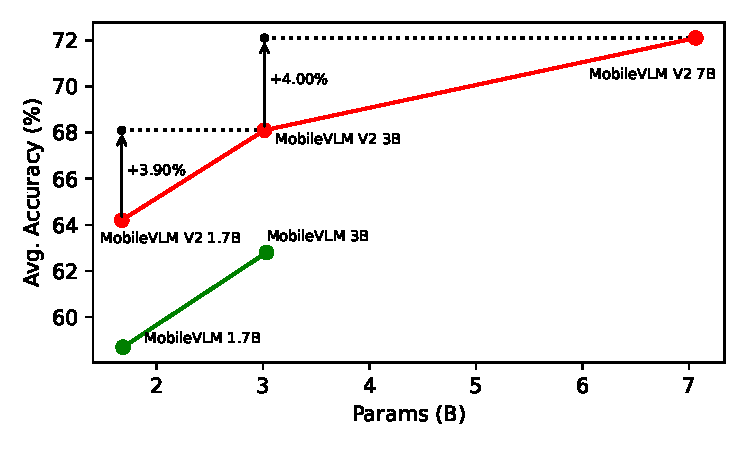
\includegraphics[width=.87\columnwidth]{figures/mobilevlm_scaling.pdf}
   \caption{Scaling of MobileVLMV2 model. As the model size increases, the performance on various benchmarks also improves, indicating the effectiveness of the model architecture and training approach.}
   \label{fig:model-scaling}
\end{figure}

\newpage

\subsection{Vision Models}

Camera team is responsible for the integration and calibration of the Mech-EYE and Intel Realsense cameras. 
They ensure that the visual data captured by these cameras is accurately processed and made available for the VLMs.
Camera team also works on optimizing the camera settings to enhance image quality and depth perception, which are crucial for effective code generation.
The main tasks of camera team is to develop a custom Vision model that can accurately detect and recognize objects in the robot's environment and provide relevant visual information to support the VLMs process.
We plan to use YOLOv11\cite{yolo11_ultralytics} as the base model for our vision tasks due to its balance between speed and accuracy. The model will be fine-tuned on our custom dataset of industrial objects to improve its performance in the specific context of robot arm applications.
The vision model will be integrated into the system to provide real-time object detection and recognition capabilities, which are essential for generating accurate and context-aware code.

However, we later found out that the YOLOv11 model was too large and computationally intensive for our limited hardware resources. Then we decided to switch to a custom lightweight model based on MobileNetV2\cite{sandler2018mobilenetv2} architecture.
This model was an experimental model that our team leader developed when he worked at FPT University AiTA-lab\cite{aita_lab}, which was optimized for speed and efficiency while still maintaining a reasonable level of accuracy.

\subsubsection{Classification Experiment}

We conducted an experiment to evaluate the performance of our custom MobileNetV2-based model on a classification task. 
The experiment involved training the model on a dataset of industrial objects and CIFAR10\cite{krizhevsky2009learning} dataset to assess its accuracy and efficiency.
\begin{figure}[ht]
  \centering
  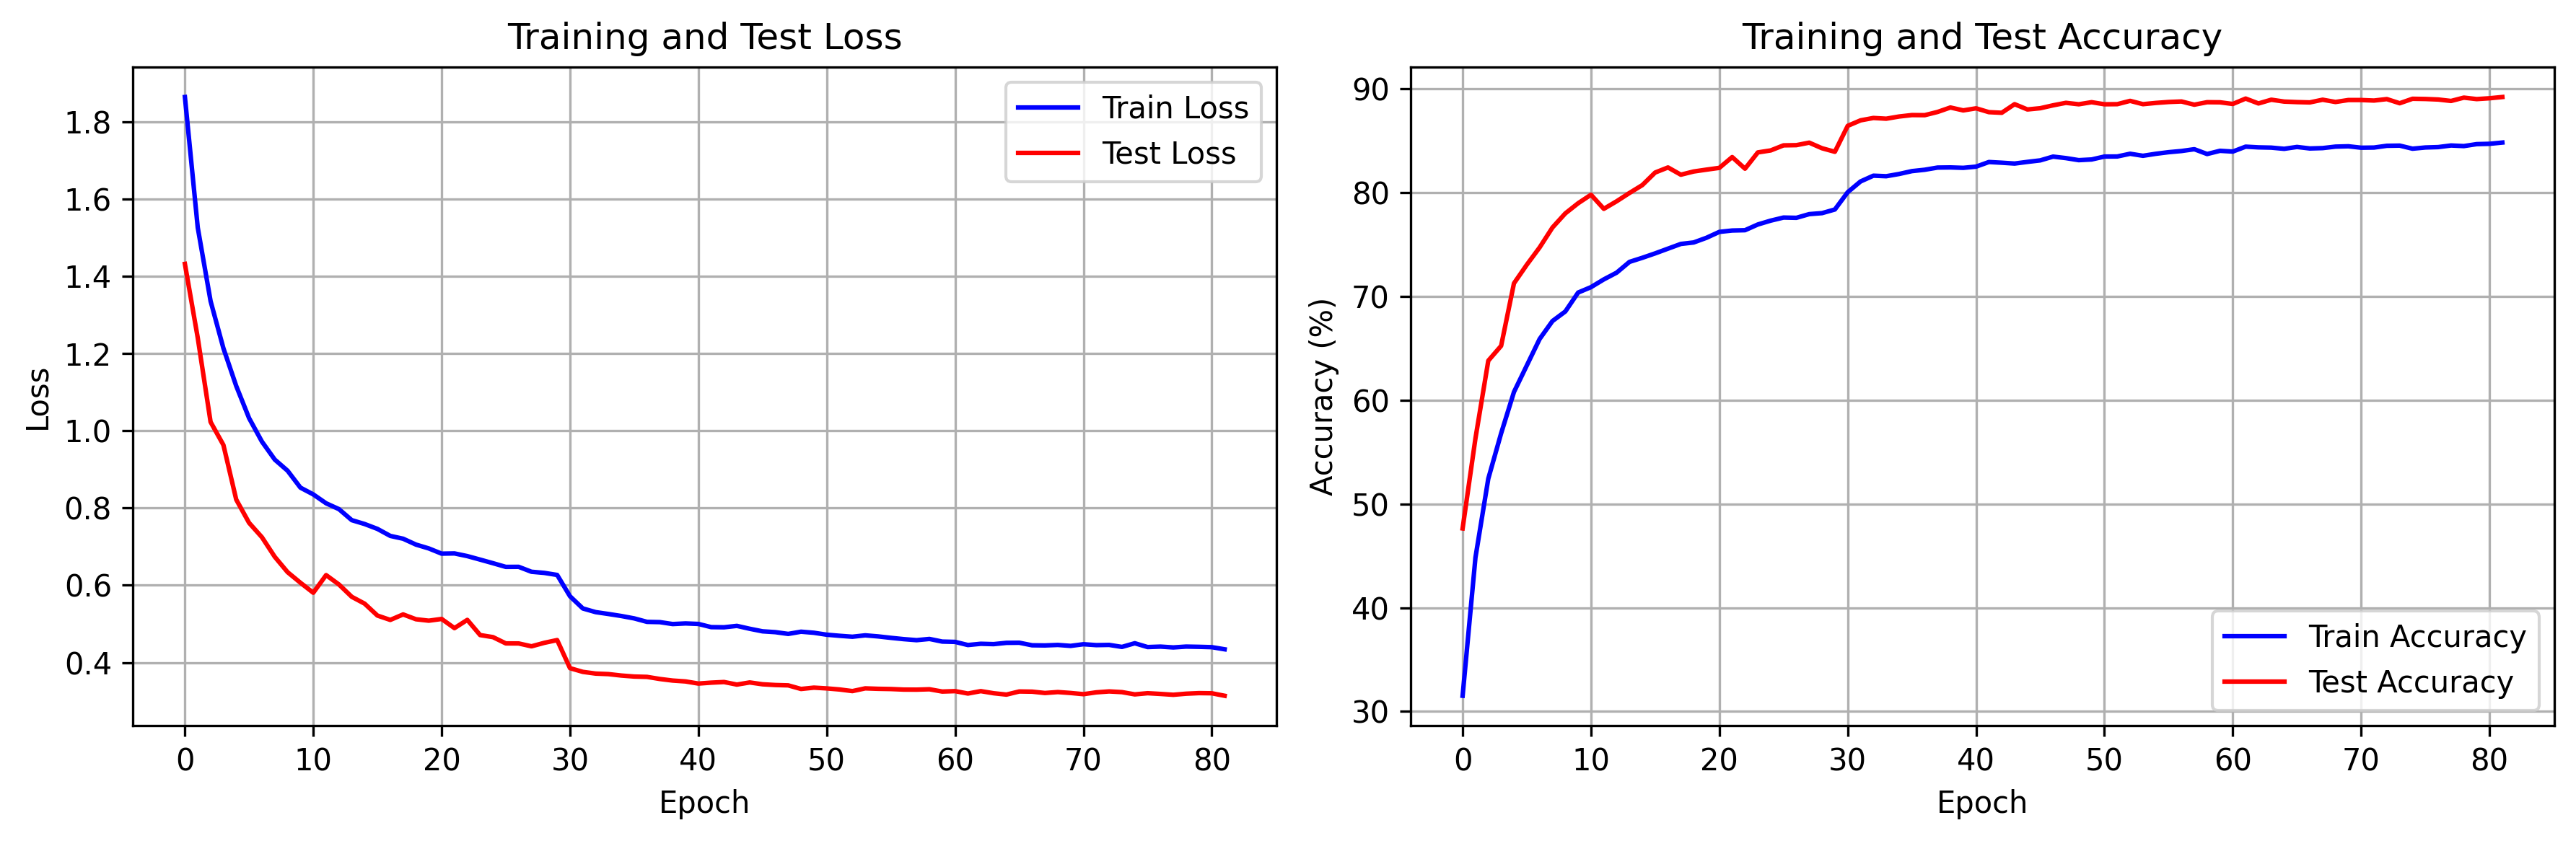
\includegraphics[width=.97\columnwidth]{340k_training_curves_postactive_W_autoaugments_2_2.png}
  \caption{Training curves of our MobileNetV2-based model on CIFAR10 datasets. The model demonstrates competitive performance while maintaining efficient training dynamics.}
  \label{fig:training-curves}
\end{figure}

Train and test result on CIFAR10 dataset in figure \ref{fig:training-curves} shows the training curves of our MobileNetV2-based model on the CIFAR10 dataset. 
This model have 0.34M parameters and 0.06 GFLOPs, which is significantly smaller and more efficient than many state-of-the-art models while it manintains competitive performance.
The small size and low computational requirements of our model make it suitable for deployment on devices with limited resources, such as embedded systems used in robotics and it illustrates the abilities of cost-effective models in real-world applications.

\subsubsection{Object Detection Experiment}

We also conducted an experiment to evaluate the performance of our custom MobileNetV2-based model on an object detection task.
We used the Pascal VOC\cite{everingham2010pascal} dataset for this experiment, which is a widely used benchmark for object detection tasks.
Model was modified by added \textbf{SSD(Single Shot MultiBox Detector)} head on top of the MobileNetV2-based backbone to enable object detection capabilities.


\subsection{Datasets}

We planned to use a combination of publicly available datasets and custom datasets tailored to our specific robotic tasks. However, the data collection process was difficult, most of the detailed robotic datasets were closed and owned by large companies. So we decided to use COCO\cite{DBLP:journals/corr/LinMBHPRDZ14} and Pascal\cite{everingham2010pascal} VOC for the vision model development process.
The model would then be fine-tuned on a more specific dataset of industrial objects that we thought would appear in normal working conditions.
Overall, this project is experimental in nature, so we will limit the variety of objects to suit the limited time and resources available.
For the VLMs for generating the robot code, we plan to reuse pretrained models with fine-tuning on a smaller dataset of robotic tasks if needed. This approach allows us to leverage the knowledge already embedded in the models while adapting them to our specific application.


\section{Results and Discussion}

\section{Conclusion}

\appendices
\section{Details of the Code Generation Pipeline}
DUMP TEXT

\section{Additional Figures}
DUMP TEXT

\bibliographystyle{IEEEtran}
\bibliography{References}
\vspace{12pt}
\end{document}